
\documentclass{article}

\usepackage{amsmath}
\usepackage{amsfonts}

\usepackage{tikz}

\begin{document}

\begin{figure}
\resizebox{\textwidth}{!}{%
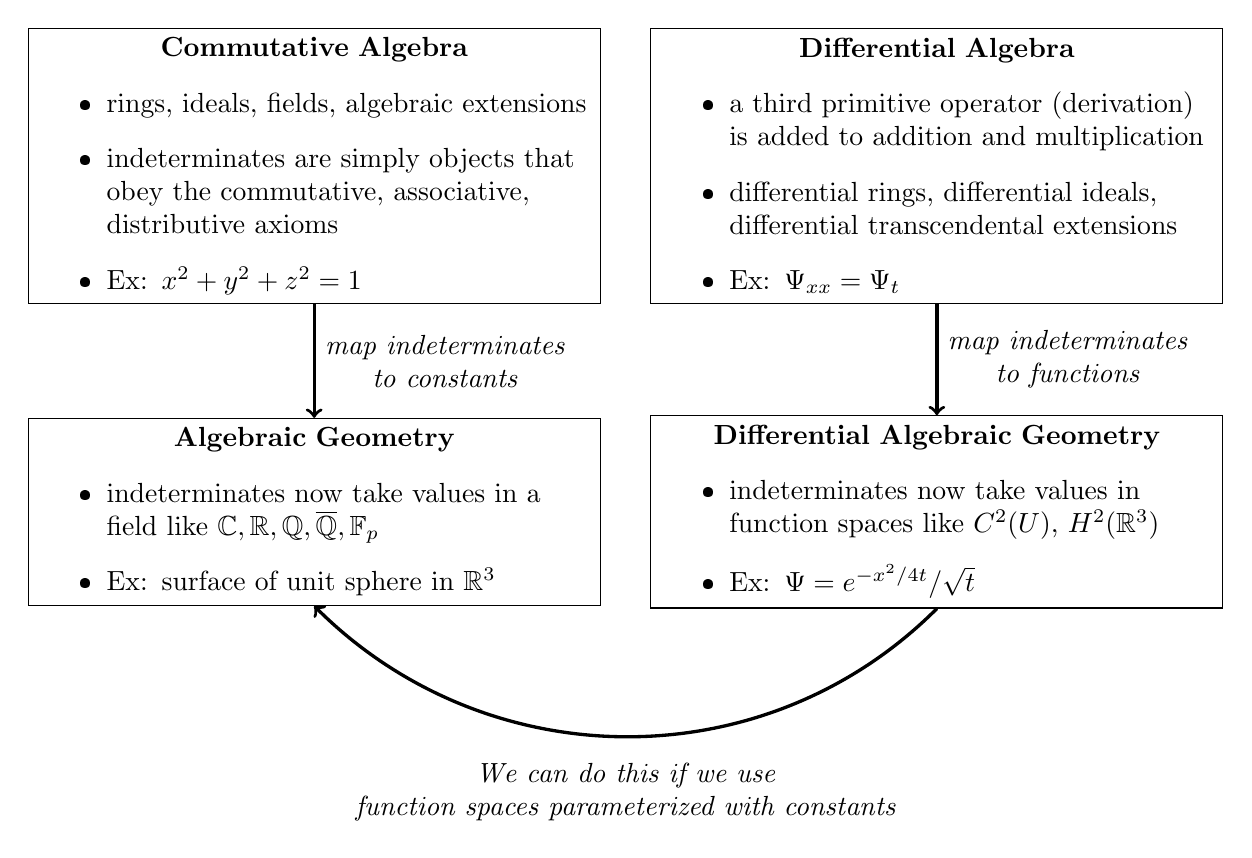
\begin{tikzpicture}[node distance=50pt, every text node part/.style={align=center}]
\node (commutative algebra) [draw, text width=200pt] {{\bf Commutative Algebra}
      \begin{itemize}
        \item rings, ideals, fields, algebraic extensions
        \item indeterminates are simply objects that obey the commutative, associative, distributive axioms
        \item Ex: $x^2+y^2+z^2=1$
      \end{itemize}
};
\node (algebraic geometry) [draw, node distance=125pt, below of=commutative algebra, text width=200pt] {{\bf Algebraic Geometry}
      \begin{itemize}
        \item indeterminates now take values in a field like $\mathbb{C}, \mathbb{R}, \mathbb{Q}, \overline{\mathbb{Q}}, \mathbb{F}_p$
        \item Ex: surface of unit sphere in $\mathbb{R}^3$
      \end{itemize}
};
\node (differential algebra) [draw, node distance=225pt, right of=commutative algebra, text width=200pt] {{\bf Differential Algebra}
      \begin{itemize}
        \item a third primitive operator (derivation) is added to addition and multiplication
        \item differential rings, differential ideals, differential transcendental extensions
        \item Ex: $\Psi_{xx}=\Psi_{t}$
      \end{itemize}
};
\node (differential algebraic geometry) [draw, node distance=125pt, below of=differential algebra, text width=200pt] {{\bf Differential Algebraic Geometry}
      \begin{itemize}
        \item indeterminates now take values in function spaces like $C^2(U)$, $H^2(\mathbb{R}^3)$
        \item Ex: $\Psi = e^{-x^2/4t}/\sqrt{t}$
      \end{itemize}
};

\draw [very thick, ->] (commutative algebra.south) -- (algebraic geometry.north) node[right,pos=0.5] {\it map indeterminates\\\it to constants};
\draw [very thick, ->] (differential algebra.south) -- (differential algebraic geometry.north) node[right,pos=0.5] {\it map indeterminates\\\it to functions};

\draw [very thick, ->] (differential algebraic geometry.south) to[out=-135, in=-45] coordinate[midway] (mid) (algebraic geometry.south) ;

\node [below of=mid, node distance=20pt] {\it We can do this if we use\\\it function spaces parameterized with constants};

\end{tikzpicture}%
}
\caption{The interrelation between four relevant branches of mathematics}
\label{concept figure}
\end{figure}

\end{document}
